\section{Future Work}
\label{sec:future}

\subsection{Improvements to the Application}
\label{sec:improvements}

In light of the evaluation, there are several improvements that could be made to the application.

\subsubsection{Background Subtraction Algorithm}

One of the points raised in the evaluation was that the model would sometimes stray from the figure whilst tracking. This seemed to be due to fluctuations in the lighting of the room. Most gyms have even lighting, but the ambient lighting would gradually change over time (for example the sun outside emerging from clouds), causing the background pixels to change their colour.

This issue could be addressed by using a more adaptive background subtraction algorithm. One proposal for this algorithm is to take the pixels that have been determined not to be foreground, and updating these pixels in the background model to a weighted average of the previous value and the new value. This would give us a background model which changes over time, allowing for gradual changes in lighting.

Another point raised in the evaluation was the difficulty in using the application in a busy gym during peak times. The application is robust to a certain degree of movement in the background during the tracking and analysis phase, meaning that a figure walking into view or performing an exercise in the background will not effect it too much. However when the application first loads, it must be placed in a still location, and in order to check that the application is still, it uses the camera to make sure that there is no motion in the feed. This means that the application must point to a clear area in order to start.

An option to avoid this requirement in the detection phase might be to switch off the motion detection and allow the user to start the processing at any time. This would not be as intuitive, as the user will not be as well informed that the phone must be placed in a still location.

Another option might be to use the Android API to access the accelerometer of the mobile device, checking its readings to detect when the device is set up correctly.

\subsubsection{Squat Rack}

Many lifters will perform their squats within the squat rack, which provides bars to catch the weight should they fail to execute the lift. These bars obstruct the view of the lifter, and therefore the current tracking algorithm cannot follow a lifter inside the rack. Figure~\ref{fig:squatrack} shows the application failing to track the lifter inside a squat rack.

\begin{figure}[H]
    \centering
    \subfigure{
            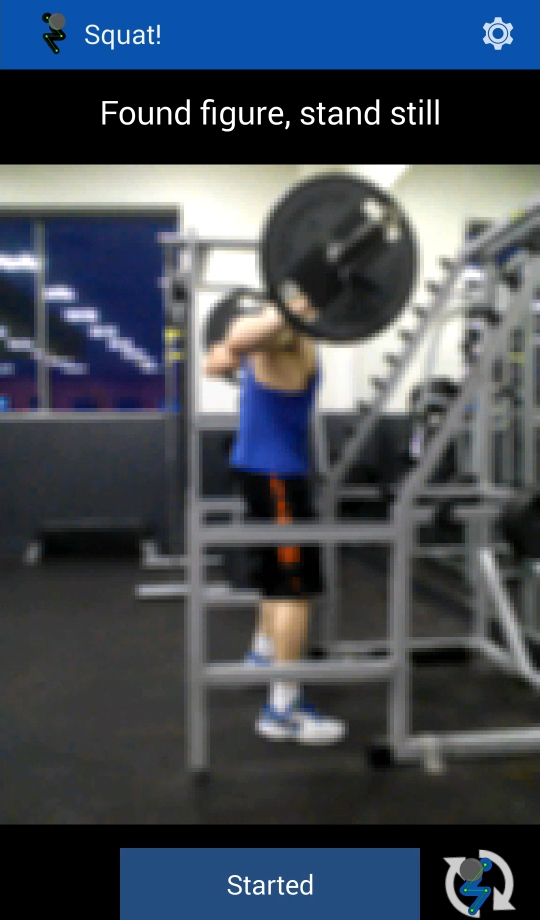
\includegraphics[height= 9cm]{future/images/squatrack}
    }
    \subfigure{
            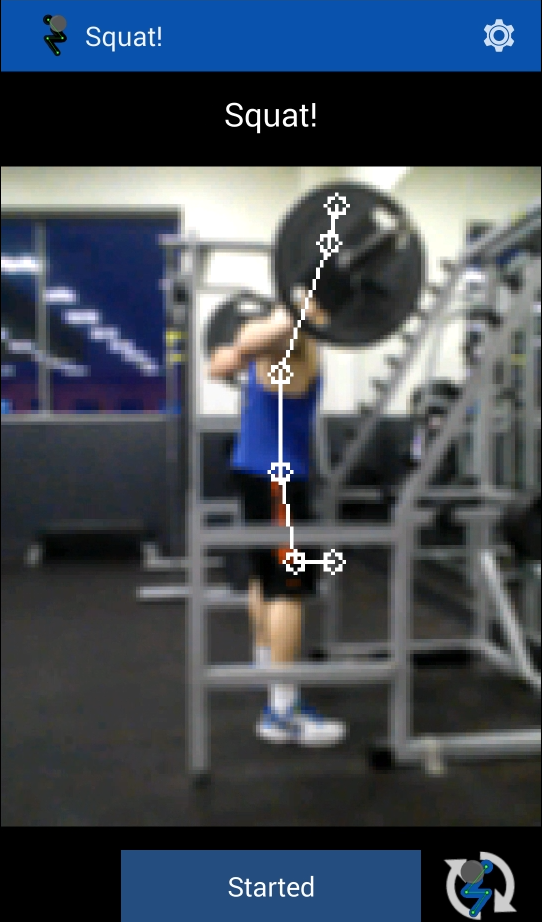
\includegraphics[height= 9cm]{future/images/squatrackfail}
    }
\caption{Tracking fails with stationary obstructions such as a squat rack}
\label{fig:squatrack}
\end{figure}

This is not a major problem, as many lifters will be happy to perform their lifts away from the rack, especially during training when lifting weights that the lifter knows they will not fail with. When a lifter attempts a new personal record, or a weight they are unsure that they are able to lift, they will use the squat rack. In this case they would not be able to use the application.

A future enhancement to the application would be to adjust the algorithm to allow for stationary objects in front of the lifter. One option which might allow for this may be to ``join'' objects detected as foreground that are reasonably close to one another, so as to create a full figure from the parts of the figure that can be seen.

\subsubsection{Resolution}

At present the resolution of the application is fairly low. Higher resolutions were tested, but the increased number of pixels reduced the reliability of background subtraction, often causing the figure to be segmented and poorly tracked.

The primary disadvantage of a low resolution is the low quality of the frames displayed to the user. In order to maintain the performance of background subtraction and the speed increase of processing fewer pixels, a future extension might be to display higher quality frames than are actually being processed. The algorithm could run on low quality frames, whilst displaying the model scaled to fit to the larger frame. This would have a minimal impact on the speed of the application, and no impact on the tracking, and provide the user with higher quality frames to give the application a more professional feel.

\subsubsection{Model Proportions}

The model is scaled to fit the lifter using a single scale factor, determined during the detection phase of the algorithm. Whilst this single scale factor adjusts the size of the model to fit the lifter, it does not adjust the model's proportions.

Through user testing, it was found that tracking is fairly robust for users with different proportions. However tracking could be improved by adjusting the models proportions to fit the lifter. It is a difficult challenge in computer vision to find the lifter's joints in order to automatically set the model's proportions, but this is something that could be investigated further to provide a more intuitive experience.

Another option might be to allow a user to set the model's proportions in the settings. This could be a simple process of inputting measurements (which would require a tape-measure) or perhaps a more interesting way would be to prompt the user to take a photo of themselves side-on using their mobile device, and have them mark their joints by tapping each joint location. The model could be drawn onto the screen as they tap, and the user could drag the joints to fine tune them once finished.

As well as proportions length-wise, the model's stature could also be adjusted in the settings. This may provide better tracking and analysis for lifters of varying weight.

\subsubsection{Model Degrees of Freedom}

Another future enhancement to the application might be the introduction of a more advanced model. The model currently has 5 degrees of freedom that the optimiser will use to adjust the model to fit the figure. This works well in practice, and gives enough information to analyse the majority of factors affecting squat form.

The spine is currently modelled as a rigid line from the shoulder/neck area to the hip. Of course this is not the case in the human body, where the spine is made up of a series of vertebrae. The spine can bend in an arc both forwards and backwards, and this can occur during squats. Perhaps a model which treated the spine as a series of connected vertebrae might track the figure better. This would also provide the ability to check whether the lifter's back was rounded in a squat, which can cause injury.

An increase in the degrees of freedom will have a detrimental effect on the performance of the fitting, giving it more variables to optimise over.

\subsubsection{Recording for Further Analysis}

An interesting idea for a feature mentioned by users in section~\ref{sec:user_testing} was the notion of recording the output of the application for later viewing. This would then allow the user to review their squat form themselves, and check whether the model tracked them accurately enough to see if its feedback is genuine.

The ability to replay a squat with an overlay of a skeleton would be a very helpful way for a lifter to review their form and learn how to improve their squats. Should this be done, it may also be worth implementing more visual feedback displayed on the screen. Joints and angles of interest could be highlighted, and labels could show the particular issues with form during the lift. At present, the application shows a ``weight distribution line'' from the centre of the weight down to the lifter's feet when the weight is in an incorrect position, but this visual form of feedback could be expanded upon in line with the verbal feedback.

\subsubsection{Voice Commands}

A way in which the level of physical interaction with the application could be minimised might be through the use of voice commands. At present once the lifter has placed their device in a still location with a clear view of the lifting area, the lifter must press the ``Start'' button. They then walk into view, and are detected when they stand still in clear view. Pressing the start button could be eliminated via a ``Start'' voice command, which would mean that once the lifter has placed their device, they no longer need to physically interact with it until they have finished using it.

Instead of automatically fitting the model to the lifter after standing still and in view, the lifter could initiate the initial fitting with a voice command. This would allow the lifter to spend more time setting up for their lift, which would be particularly useful should they like to make small adjustments to the placement of their feet.

Other voice commands could be used during the squatting phase should the lifter realise they did not set their preferences as desired. For example if after their first repetition the lifter realised they did not have the sound on, they could issue a command to switch it on and continue their set with verbal feedback.

\subsubsection{Other Lifts}

As well as general enhancements to the current algorithm and application, there are many other lifts that could be introduced, each with their own factors affecting their form.

The deadlift and bench press are the other two powerlifting techniques that would be useful to analyse. Deadlifts would be particularly useful, being an advanced technique that often causes back injury due to incorrect form. A particular challenge with deadlifts might be that the bar is usually placed in the lifting location prior to the lifter entering the scene. This is unlike a squat, where the lifter and bar will enter the view together. With the current algorithm, the bar would be detected as background whilst on the ground, and only as foreground once it left the ground. A very similar model could be used, only requiring the addition of arms to the current model used for squats.

The bench press would come with other challenges. A different viewpoint may be required to check whether the lift has been executed correctly - factors such as the position of the bar along the lifter's body, the angle of the lifter's elbows, whether the bar touched the lifter's chest, and many others cannot all be determined from the same viewpoint.

Other lifts that this technology could be applied to are the Olympic weightlifting techniques. The two Olympic weightlifting techniques are the ``clean and jerk'' and the ``snatch''. These lifts are more complicated than the powerlifting techniques, with several stages to each lift with the goal of raising the bar above the lifter's head. Each of these lifts however could be monitored side-on with a monocular camera to check the majority of factors determining the safety and validity of the lift. Whilst powerlifting techniques are used a lot in general training at the gym (whether for sport or recreationally), Olympic weightlifting techniques are more commonplace in a professional environment. This might mean that there is scope for other methods such as the use of a stereo camera or Kinect to separate the lifter from their surroundings, and to track the technique in a three-dimensional way. 

\subsubsection{Social Network}

Perhaps another future enhancement to this application would be to build a social network around it. This could allow users to share scores and compete with one another, encouraging them to work on their squat form and to keep training at the gym.

This idea could be taken even further, with the possibility of sharing videos of their tracked squats. This way lifters would be able to receive feedback from a community of gym-goers as well as from the analysis of the application. Human observers would be able to provide a more accurate critique of squat form, and will be able to pick up on errors that are too subtle to be detected by the application.

This would enrich the overall user experience of the application, and provide users with even better feedback.

\subsection{Launch}

In the not too distant future, I aim to launch the application to the general public, placing it on the Google Play\cite{googleplay} store. The application is in a good state to release immediately, but some of the improvements mentioned in section~\ref{sec:improvements} may be added prior to launch.

There has been some online interest in the application since I uploaded a video demonstration of the application to YouTube\cite{youtube}. Particular interest was shown on a few threads on Reddit\cite{reddit}\cite{redditpopularity}, which linked to the video. Comments included:

\begin{quote}
\emph{Give me this already!}
\end{quote}

\begin{quote}
\emph{I'd love to see this and one for deadlifts!}
\end{quote}

\begin{quote}
\emph{This is phenomenal, and I wish it were almost required at some gyms. I see some kids doing some nasty Squats that they are gonna regret when they get older.}
\end{quote}

From these comments and many more, it can be seen that this application will be very useful, and I look forward to launching it and continuing to develop it in the future.

\subsection{Other Applications}

The technology used in this project has applications outside of weight lifting, in both sports and other areas.

\subsubsection{Sports}

Within sports there is a very wide scope for figure tracking and analysis.

One particular application might be for cyclists training on a rolling road. A particularly important part of the cyclist's technique is to keep their torso close to the bike to minimise drag. Tracking and analysis could be used to determine whether the cyclist is in the correct position, indicating when they rise up into a sub-optimal position in real-time.

There is also scope for use in gymnastics, where weight distributions could be analysed to aid gymnasts in their technique, prompting them to lean more in a particular direction.

\subsubsection{Other Fields}

Other uses for real-time body tracking might be in interaction with user interfaces and games. Kinect already shows the popularity of this kind of technology, but this is lacking in the mobile industry. This technology could be applied to interacting with the interface of a mobile phone via the use of gestures, or perhaps in a game to allow you to adjust the pose of a character by moving your own body.

